\section{Experimental Results}
\label{sec:experiments}

\noindent
\textbf{Overview.}~ We first explain with an example how the 
problem of finding 
predecessors can be expressed as a SAT problem.
We then discuss our experimental results.
All of our experiments used the SAT-based approach for finding
predecessors.

\smallskip

\noindent
\textbf{Reducing Predecessor Finding to SAT:}
We now discuss  a method to convert the problem of finding one or more
predecessors of a given configuration of a SyDS into a general form 
of the Boolean Satisfiability problem. 
This method converts the predecessor 
problem into an expression of
the form $F_1 \wedge F_2 \wedge \ldots \wedge F_r$, where each
component $F_j$ ($1 \leq j \leq r$) is a Boolean subexpression,
which need not be a clause (i.e., disjunction of literals).
Methods are known for converting any Boolean subexpression
into its CNF equivalent.
As a consequence, SAT solvers 
can be used to solve the predecessor problem. 

We assume that the nodes of the underlying graph of the
given SyDS are numbered 1 through $n$ that
and the local function at node $i$ is denoted by $f_i$,
$1 \leq i \leq n$.
For each node $i$, $N_i$ denotes the \textbf{closed neighborhood}
of node $i$ (defined in Section~\ref{sec:prelim})
in the underlying graph; thus, the states of the nodes in $N_i$ 
are the inputs to the local function $f_i$,
$1 \leq i \leq n$.

\smallskip

Recall that the predecessor existence problem asks whether a given
configuration \calc{} of a given SyDS \cals{}
has a predecessor, that is, a configuration \calcp{} such that 
\calc{} is the successor of \calcp.
If so, we want to find one such configuration.
Let \calc{} = $(c_1, c_2, \ldots, c_n)$ be
the given configuration for which we need to 
find a predecessor (if one exists).
Note that each $c_i$ is a known 0 or 1 value, $1 \leq i \leq n$.
We need to find a configuration 
$\calcp{} = (x_1, x_2, \ldots, x_n)$ such that \calcp{}
is a predecessor of \calc{} (if one exists). 
As before, this condition can be expressed as a SAT problem as follows.

Consider node $i$ of the SyDS. 
As mentioned earlier, let $N_i = \{i_1, i_2, \ldots, i_r\}$
denote the closed neighborhood of node $i$, where $r = |N_i|$.
Thus, the inputs to the local function $f_i$ at node $i$
are $x_{i_1}$, $x_{i_2}$, $\ldots$,  $x_{i_r}$.
Since we want \calcp{} to be a predecessor of \calc, the condition to
be satisfied at node $i$ is:
\begin{equation}\label{eqn:pre_cond_one}
     c_i  ~\Leftrightarrow~ f_i(x_{i_1}, x_{i_2}, \ldots,  x_{i_k})
\end{equation}
Since $c_i$ is a known 0 or 1 value, the expression given 
in Equation~\eqref{eqn:pre_cond_one} can be simplified.
If $c_i = 0$, it can be seen that the above expression 
simplifies to $\neg\,f_i(x_{i_1}, x_{i_2}, \ldots,  x_{i_k})$.
Likewise, if $c_i = 1$, the above expression 
simplifies to $f_i(x_{i_1}, x_{i_2}, \ldots,  x_{i_k})$.

Using $P_i$ to denote the subexpression given by Equation~\eqref{eqn:pre_cond_one}
for node $i$, the condition to be satisfied for \calcp{} to be a 
predecessor of \calc{} is given by 
\begin{equation}\label{eqn:pre_whole}
P_1 ~\wedge~ P_2 ~\wedge~ \ldots ~\wedge~ P_n
\end{equation}
As before, since each subexpression $P_i$ can be expressed as an equivalent CNF, 
we can get a CNF formula with variables $x_1$, $x_2$, $\ldots$, $x_n$
from Equation~\eqref{eqn:pre_whole}. 
Each solution to the resulting CNF formula (which can be obtained using
a SAT solver) gives a predecessor of the given configuration \calc.
If there is no satisfying assignment to the CNF formula corresponding
to the expression in Equation~\eqref{eqn:pre_whole}, then \calc{}
has no predecessor; that is, \calc{} is a Garden-of-Eden configuration.

%%\medskip

\begin{figure}[tbh]
%%\rule{\textwidth}{0.01in}
%\medskip
\begin{minipage}{0.5\textwidth}
\centering
%\hspace*{1in}
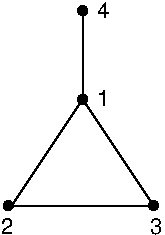
\includegraphics[scale=0.75]{./graph_example.pdf}
\end{minipage}
\hspace*{0.25in}
\begin{minipage}{0.4\textwidth}
%%\underline{\textsf{Local Functions:}}
\smallskip
\noindent
\begin{tabular}{|c|c|}\hline
\textbf{Node} & \textbf{Function} \\ \hline
1  &  OR \\ \hline
2  &  AND \\ \hline
3  &  NAND \\ \hline
4  &  NOR \\ \hline
\end{tabular}
\end{minipage}
\caption{\small{SyDS Example used to illustrate
the conversion predecessor problem to SAT.}}
\label{fig:syds_ex}
%%\rule{\textwidth}{0.01in}
\end{figure}
%%

\noindent
\textbf{Example:} Consider the SyDS example shown in Figure~\ref{fig:syds_ex}.
Suppose we want to find a predecessor of the configuration $(1, 0, 1, 0)$.
Using $x_1$, $x_2$, $x_3$ and $x_4$ to denote the Boolean variables corresponding
to the nodes 1, 2, 3 and 4, the Boolean formula to be satisfied when 
$(x_1, x_2, x_3, x_4)$ is a predecessor of $(1, 0, 1, 0)$ is:  

\medskip

\noindent
\hspace*{0.5in} $[1 ~\Leftrightarrow~ \mathrm{OR}(x_1, x_2, x_3, x_4)] ~\wedge~
[0 ~\Leftrightarrow~ \mathrm{AND}(x_1, x_2, x_3)] ~\wedge~ $\\
\hspace*{0.5in}
$[1 ~\Leftrightarrow~ \mathrm{NAND}(x_1, x_2, x_3)] ~\wedge~
[0 ~\Leftrightarrow~ \mathrm{NOR}(x_1, x_4)]$

\smallskip

\noindent
The above expression can be simplified to:

\begin{center}
$[\mathrm{OR}(x_1, x_2, x_3, x_4)] ~\wedge~
[\neg\,\mathrm{AND}(x_1, x_2, x_3)] ~\wedge~ 
[\mathrm{NAND}(x_1, x_2, x_3)] ~\wedge~
[\neg\,\mathrm{NOR}(x_1, x_4)]$
\end{center}

\noindent
By converting each subexpression above into its CNF equivalent, and
noticing that the term $[\mathrm{NAND}(x_1, x_2, x_3)]$ occurs twice
in the above expression, we get the following simplified
CNF formula:

\begin{center}
$(x_1 \vee  x_2 \vee  x_3 \vee  x_4)  ~\wedge~
(\overline{x_1} \vee \overline{x_2} \vee \overline{x_3}) ~\wedge~ 
(x_1 \vee x_4)$
\end{center}

%%\medskip

\noindent
\textbf{Note:}~ Simple constraints (such as requiring
the states of some nodes to be 0 and/or those of some nodes to be 1
in the predecessor) can be handled by inserting appropriate 
single literal clauses.
For example, we require a predecessor in which node 1 is in state 0
and node 3 is in state 1, then we can add the single literal clauses
$\overline{x_1}$ and $x_3$ to the resulting CNF expression.
This illustrates the usefulness of the SAT formulation.
